\documentclass[10pt,a4paper]{report}
\usepackage[latin1]{inputenc}
\usepackage{amsmath}
\usepackage{amsfonts}
\usepackage{amssymb}
\usepackage{graphicx}
\usepackage[danish]{babel}
\usepackage{hyperref}

\title{Webintelligence - Mini Project 2}
\author{Lars Andersen, Mathias Winde Pedersen \& S�ren Skibsted Als}
\begin{document}
	\maketitle
	
	\section*{Part 1 - Community Detection}
	The task of detection communities is the task of finding clusters in the friendships network.
	In order to do this, we draw upun the spectral clustering power, and we use that for finding clusters.
	
	But, before we discuss of the spectral clustering works, some theory needs to be explained.
	
	\subsection*{Unnormalized Laplacian}
	We need to be able to compute the unnormalized Laplacian matrix, which is a matrix consisting of the diagonal matrix (D) and the relationship matrix (A), constructed as $L = D - A$. Where the diagonal matrix D has numbers on the diagonal equal to the sum of numbers for that given row in the A matrix.
	An example of this can be seen in Figure \ref{fig:spectral}, where you for now can ignore the eigenvectors part.
	
	\begin{figure}[h]
		\centering
		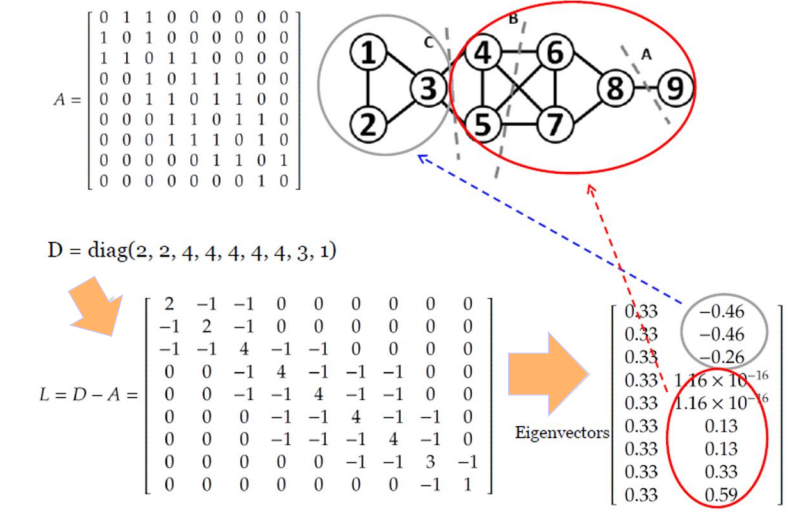
\includegraphics[scale=0.5]{spectral-cluster}
		\caption{Laplacian example}\label{fig:spectral}
	\end{figure}
	
	\subsection*{Eigen decomposition}
	Some other computations needed for the spectral clustering is the eigen vector decomposition (EVD).
	To calculate this, we used the mathnet.numerics library, as it was able to calculate the EVD multithreaded.
	What you calculate the EVD of is the unnormalized laplacian matrix.
	
	The library used was also good in the sense that the vectors were sorted according to their respective eigenvalues.
	
	\subsection*{Spectral Clustering}
	As mentioned, we used the unnormalized laplacian for our spectral clustering algorithm, resulting in a RatioCut.
	An alternative is to use the normalized laplacian, resulting in a NormalizedCut.
	However, we had no incentive to use the NormalizedCut, as that cut considers the overall structure, but this is irrelevant for us.
	
	As taken from the slides, the spectral clustering then works as follows:
	\begin{enumerate}
		\item Compute the unnormalized Laplacian $L$.
		\item Compute the second eigenvector $v:2$ of $L$ (the one with the second smallest eigenvalue - not 0).
		\item The $j$'th value in eigenvector corresponds to the $j$'th node.
		\item Order the nodes according to their eigenvector-values
		\item Cut at the largest gap
	\end{enumerate}
	For the algorithm above, the largest gap can be now be seen in Figure \ref{fig:spectral}, in the lower right corner.
	
	The results of running this community detection is that we found 4 clusters, resulting in 4 communities. 
	We also printed the relations to a png file and it also indicated 4 communities.
	
	At this point in time, when we decide enough clustering have been performed, we use a threshold for the largest gap, and just decide on this.
	In the future, with more time, we would used the Modularity of the clusters for this.
	The idea of modularity is that in a real.world scenario, modularity is a measure of how much the edges in the graph falls withing the same cluster, opposed to a randomly across clusters, see the slides.
	
	\section*{Part 2 - Sentiment Classifier}
	The idea of having a sentiment classifier for this miniproject, is that based on a review, we are able to tell whether the review is positive or negative.
	The baseline of the algorithm is the following: (taken from slides)
	
	\begin{itemize}
		\item Tokenization
		\item (Stemming usually not good for sentiment analysis)
		\begin{itemize}
			\item Sometimes destroys the Positive/Negative distinction
		\end{itemize}
		\item Feature Extraction
		\item Classification using different classifiers
		\begin{itemize}
			\item Naive Bayes
			\item MaxEnt
		\end{itemize}
	\end{itemize}
	Each of these relevant parts will be described in turn.
	
	\subsection*{Tokenization and feature extraction}
	For the tokenization, we used the proposed python library (Potts) and translated it into c\#, such that it was easily available for use in our visual studio project.
	The library takes care of splitting the string into tokens, and in that regard uses several useful regex's, and also takes care of handling negation by adding a "not" suffix to each token. Another powerful token to recognize with this is capturing emoticons, which the library also takes care of.
	
	The tokenization and feature extraction is somewhat merged into one here, as the handling of negation and such is part of feature extraction, but is handled by the implemented tokenizer.
	
	\subsection*{Classification}
	For the classification, which for us consist of prediction whether a review is positive or negative, can use several algorithms.
	We decided to use the Naive Bayes algorithm, as it is known to do decently well, although simple.
	
	In order to predict the classification of reviews, training data is used.
	For the training data, you have  a review and its associated score, which is used to calculate the probabilities for being positive and negative for each of the tokens.
	
	The Naive Bayes classifier, builds upon bayes theorem that says for two stochastic variables $C$ and $X$, bayes theorem says: $p(C|X) = \frac{p(X|C) * p(C)}{p(X)}$.
	
	The score for class $c\in C$ given review $x$ is:
	$$score(x,c) = p(c|x) = \frac{p(x|c)*p(c)}{p(x)}$$
	However, the division with $p(x)$ can be excluded, as that is the same for all $c$.
	 
	With the assumption that the features are independent given the class attribute.
	The score can then be calculated as follows:
	$$score(x,c) = (\prod_{i=1}^{n}{p(x_i|c)})p(c)$$
	
	And the way you then would decide on which class to pick, it is simply choosing the class with the highest score.
	
	In order to reduce the amount of computations needed we use the following trick:
	As the reviews usually contain only a small subset of the vocabulary, the following computation is much more efficient.
	$$score^*(empty, c) = (\prod_{i=1}^{n}{p(\text{not }x_i|c)})p(c)$$
	
	if you have a review $x$ consisting of the words $x_1, ...,x_k$, the score can be calculated as follows:
	$$score(x, c) = score^*(empty, c)(\prod_{j=1}^{k}{\frac{p(x_j|c)}{p(\text{not }x_j|c)}})$$
	
	Additionally, we use another trick to ensure numerical stability.
	The idea is that instead of having multiplications, which can become very large, you switch to log-space such.
	So this just uses the logarithmic rules to give you.
	$$\log score(x,c) = \log p(c) + \sum_{i=1}^{n}{\log p(x_i|c)}$$
	
	\subsection*{Learning the model}
	To learn the model, it is a matter of simple counting, with a modified Laplace smoothing.
	What you count is used to calculate the following, where $|C| = 2$ for our case, as we have two classes (positive and negative):
	$$p(c) = \frac{N(c) + 1}{N + |C|}$$
	
	The dependent probability distributions is calculated as follows:
	$$p(x_i|c) = \frac{N(x_i, c) + 1}{N(c) + |X|}$$
	Where,
	\begin{itemize}
		\item[$N(x_i, c)$] is the number of times the word $x_i$ appears across all reviews with sentiment $c$.
		\item[$|X|$] is the size of the vocabulary.
	\end{itemize}
	
	\subsection*{Corners Cut}
	We did not try and use the MaxEntropy algorithm, and could be interesting to use in the future, as the reading material states that its performance is usually better than the Naive Bayes algorithm.
	
	Additionally, we did not use the reviews that had a score of 3.0 to learn our classifier. Those reviews may have been of use, to have a neutral category or something of the like, but for this task with only two classes, we did not see how we could use it, and as of such excluded it.
	
	\subsection*{How good is the classifier}
	To determine the quality of the classifier, we used cross-validation, by splitting the data 10-fold.
	For each fold, we use that as a temporary test set, and the other 9 folds as training data, and then calculate the performance, after which we calculate the average performance of the 10 runs. This gave us an precision of about $80\%$ for positives, but we had a precision of about $60\%$ for negatives.
	We find this a good performance, considering the low complexity of the classifier.
	
\end{document}